\chapter{PX aspects, methods and instruments to evaluate \acp{PREG}}
\label{ch:aspects}

As discussed in \autoref{ch:characterising}, there are constraints that evaluators should consider when evaluating \ac{PX} in \acp{PREG}. Those aspects include common \ac{PX} aspects such as enjoyment, immersion or presence. However, since the use of a \ac{PREG} depends on its capability to meet patients' and physiotherapists' expectations and needs aspects such as safety, motivation, effectiveness, ease of use and usefulness are of high relevance. Therefore, we conducted a qualitative study with people from the physiotherapy domain to identify a set of relevant aspects that allow evaluators to assess \acp{PREG} properly. Since we used semi-structured interviews for the study, we could also identify some instruments and methods to assess the identified aspects that relate to physical rehabilitation.

%-----------------------------------
%\section{Aim of the study} % Aim of the study -----------------------------------

%-----------------------------------
\section{Materials and methods} % Materials -----------------------------------
\label{sec:mats_mets_aspects}
% Interviews (Include leading questions), observation, 
% Thematic content analysis (for qualitative research) using affinity charts
% One coder
% Validation: Review by physiotherapists 
We conducted two semi-structured interviews with a physiotherapist and an undergraduate physiotherapy student. The physiotherapist belongs to the Evaristo Garc\'ia University Hospital, in Cali Colombia, and the student participated in the development of a collection of mini \acp{PREG}. We guided the interview using the following questions:

\begin{enumerate}
    \item What should one consider when evaluating a \ac{PREG}?
    \item What aspects should one evaluate to assess the quality of a \ac{PREG}?
\end{enumerate}

Additionally, we inspected the logs of a validation process conducted by the physiotherapy student, who tested a set of mini \acp{PREG}. Those logs contained observations and recommendations regarding errors or improvements that she found. We analysed the logs to identify which aspects she considered during the validation process.

We took notes for both interviews, and the logs of the validation process were available online. We analysed the data using the thematic content analysis method \autocite{Burnard2008}. First, we produced a list of statements associated with the mentioned questions. Then, we assigned a theme to each statement to produce our initial coding framework. After that, we grouped themes to reduce the number of categories. We continued until we obtained four categories for our final coding framework. This process is illustrated in \autoref{fig:aspectsIdentification}. We presented our framework to the student and three physiotherapists to validate that our results represented their view. They clarified or added information regarding two statements.

\begin{figure}[htb]
\myfloatalign
{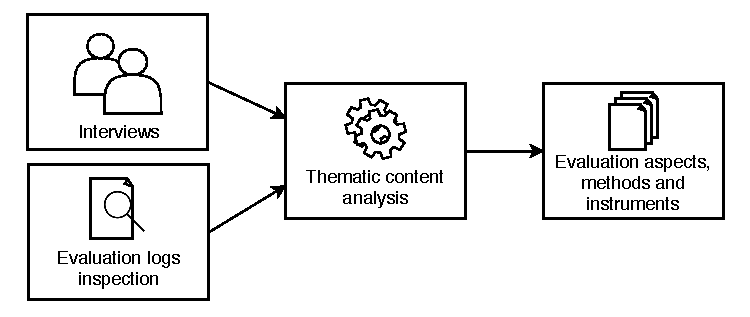
\includegraphics[width=\linewidth]{gfx/aspects/aspectsIdentification}} \quad
\caption{Aspects, methods and instruments identification process}\label{fig:aspectsIdentification}
\end{figure}

%-----------------------------------
\section{Findings} % Findings -----------------------------------
\label{sec:findings_aspects}

We identified 59 statements regarding aspects, instruments and methods to evaluate \acp{PREG}. After grouping and categorising the statements iteratively, we identified four final categories: evaluation aspect (37 statements), evaluation instrument (14 statements), evaluation method (7 statements) and evaluation occurrence (1 statement).

\subsection{Evaluation aspects}
\label{sec:rehab_aspects}
According to the physiotherapists, the main reason to include games in rehabilitation therapies is to increase patient’s \textit{motivation} towards their therapy. Physiotherapists considered important that \acp{PREG} offer a balance between game challenges and patients skills. Thus, evaluators should evaluate aspects such as challenge \autocite{Moosajee,Nacke2009,VandenAbeele2016,Wiemeyer2016,Desurvire2009} and flow \autocite{Sinclair2007,Lapas2015,Bernhaupt2015,Nacke2009,Wiemeyer2016,Nijholt2008}. Also, patient's emotions while playing are important to keep them motivated. Thus, emotion \autocite{Bernhaupt2015,Sanchez2009,Wiemeyer2016}, engagement \autocite{Yanez-Gomez2017,Wiemeyer2016}, negative-positive affect \autocite{Nacke2009}, interest \autocite{VandenAbeele2016} and enjoyment \autocite{Ho2017,Li2016,VandenAbeele2016,Zhao2016,Li2006,Berkovsky2010} are relevant aspects.

Physiotherapists remarked that the highest expectation of patients is to finish their therapies as soon as possible to return to their daily life activities. As a result, when a physiotherapist includes something new into the therapy, patients expect it to be meaningful to their rehabilitation progress. Therefore, evaluators should evaluate the capability of \acp{PREG} to contribute to the achievement of the rehabilitation goal. It can be assessed by evaluating rehabilitation aspects that indicate the achievement of the sought goal. Those aspects include balance, flexibility, the range of motion, strength, resistance, dyspnea (shortness of breath), pain, \ac{HR}, oxygen saturation, functional independence, proprioception and motor coordination.

Furthermore, physiotherapists highlighted that \acp{PREG} should guarantee \textit{patients' safety}, i.e., those cannot produce any injury, hurt or loss to patients. Patients' safety may be assured by allowing to personalise and configure game sessions to meet their needs. Configuration parameters include gameplay time or the number of repetitions, movements selection, movement range and speed. 

After analysing the student's validation logs, we concluded that correctness and understating of configuration parameters are relevant evaluation aspects. Correctness means that configuration parameters produce the expected behaviours. If the \ac{PREG} is supervised, those parameters should be understandable for physiotherapists, or for patients if it is unsupervised. Also, those parameters should cover all movements associated with the \ac{PREG}. The correctness of parameters may be assessed by physiotherapists.

Furthermore, a \ac{PREG} has to enable \textit{adaptation} to patients particular needs while they are playing \autocite{Cameirao2010,Ni2014,Nijholt2008,Wiemeyer2015}. If the \ac{PREG} is supervised, that process is automatic and may involve a movement monitoring system. Otherwise, adaptation is performed by physiotherapists and the \ac{PREG} should facilitate re-configuring parameters during gameplay.

Both the physiotherapists and the student's logs suggested that some aspects regarding the \textit{associated movements} of a \ac{PREG} are important. First, movement mapping correctness should be assured since \acp{PREG} use patients' body movements to enable interaction. Second, all movements should be covered by the game mechanics. Also, patients should consider those movements as meaningful; i.e., the movements should be aligned with the game goals. Evaluators can consider aspects such as accomplishment \autocite{Cameirao2010,Zhao2016} and clarity of game goals \autocite{Desurvire2009,VandenAbeele2016}. Third, movement correctness monitoring should be enabled or facilitated by the \ac{PREG}. If the \ac{PREG} is unsupervised, feedback about movement correctness should be automatic, immediate, realistic and specific. Otherwise, physiotherapists should be able to interrupt gameplay to correct patients. Finally, the point of view of the \ac{PREG} should allow patients to identify the outcomes of their actions easily.

We also found that \acp{PREG} should be \textit{easy and natural to use}. Thus, evaluators should assess aspects such as cognitive load and attention. The \ac{PREG}’s cognitive load should not distract patients from the expected rehabilitation goal. Patients’ attention should be focused on achieving game goals and not on learning how to control the \ac{PREG}. Additional aspects to be evaluated would be learnability \autocite{Desurvire2009,GonzalezSanchez2009} and absorption \autocite{Lapas2015}. Additionally, \acp{PREG} can include tutorials, which should be complete and understandable. A tutorial is complete if it covers all associated movements and explains their relation to game mechanics. It should be understood by physiotherapists and patients.

Furthermore, the physiotherapists expressed that \acp{PREG} should offer \textit{feedback about progression}. That includes performance measurements per session like the maximum achieved movement angles or the number of correct executed movements.

Finally, evaluators should consider monitoring a group of patients throughout their whole rehabilitation treatments to asses a \ac{PREG} properly. Also, health instruments and the participation of physiotherapists may be required.

\subsection{Evaluation methods}
\label{sec:rehab_methods}
The interviews allowed us to identify the following three types of methods for evaluating rehabilitation aspects: 

\begin{enumerate}
  \item \emph{Physiotherapist observation}: the evaluation of an aspect depends on the physiotherapist's observation and the criteria of the instrument being employed. For instance, when physiotherapists assess the balance of a patient using the flamingo test \autocite{flamingo}. 
  \item \emph{Self-reported}: patients rate an aspect subjectively, and physiotherapists establish conclusions according to the employed instrument. For instance, patients rate the pain intensity they are feeling using a \ac{VAS} \autocite{vasScale}.
 \item \emph{Physiological}: physiotherapists collect data directly from patients body; e.g. when they measure the range of motion of a joint.
\end{enumerate}

\subsection{Evaluation instruments}
\label{sec:rehab_instruments}
The interviews also allowed us to identified some physiotherapy instruments that can be used to evaluate some of the rehabilitation aspects mentioned above. Interviewed physiotherapists expressed that they use the Daniels \autocite{danielsScale}, the \ac{MAS} \autocite{ashwortScale}, the Kendall \autocite{kendallScale}, the Oxford \autocite{oxfordScale} and the \ac{MRC} \autocite{mrcScale} scales to assess muscle strength. They measure pain using the \ac{VAS} \autocite{vasScale}, the \ac{FLACC} \autocite{flaccScale} and the Wong-Baker FACES \autocite{Baker} scales. Also, they use the pulse oximeter to measure \ac{HR} and oxygen saturation. They use the Modified Borg Scale \autocite{modifiedBorgScale_2014} to assess dyspnea, i.e., shortness of breath, and perceived exertion. Finally, they expressed that they used the \ac{FIM} \autocite{fim} to assess patients' functional independence and the goniometer \autocite{goniometry} to measure the range of motion. 

Furthermore, the physiotherapists mentioned three tests to assess balance; i.e., the flamingo test \autocite{flamingo}, the tandem gait test \autocite{tandemGaitTest} and the stork test \autocite{storkTest}. One physiotherapist said that they use the floor touch test \autocite{floorTouch} to assess flexibility. 

The selection of instruments depends on the rehabilitation goal of the evaluated \ac{PREG}. Also, some instruments are of private use, which means that each health institution may have different instruments.

\subsection{Evaluation occurrence}
The physiotherapists expressed that evaluations occur before, during and after therapies take place. That allows diagnosing patients health status and track their progress. 

% -----------------------------------------------
\section{Discussion} % Discussion %-----------------------------------------------
\label{sec:discussion_aspects}

The aim of this study was to identify aspects that physiotherapists consider important to evaluate \acp{PREG}. Based on the findings, it is confirmed that there are rehabilitation aspects that evaluators should consider to assess the impact of \acp{PREG} on patients' therapies. We identified a set of aspects related to motivation, rehabilitation goal achievement/support, patients' safety, adaptation, associated movements, ease of use and patient's progress feedback. All those aspects are relevant to assess if a \ac{PREG} meets physiotherapists and patients needs, which is relevant to include it as an assisting methodology in a therapy.

Our study confirmed that common evaluated \ac{PX} aspects such as challenge \autocite{Moosajee,Nacke2009,VandenAbeele2016,Wiemeyer2016,Desurvire2009}, flow \autocite{Sinclair2007,Lapas2015,Bernhaupt2015,Nacke2009,Wiemeyer2016,Nijholt2008}, emotion \autocite{Bernhaupt2015,Sanchez2009,Wiemeyer2016}, engagement \autocite{Yanez-Gomez2017,Wiemeyer2016}, negative-positive affect \autocite{Nacke2009}, interest \autocite{VandenAbeele2016} and enjoyment \autocite{Ho2017,Li2016,VandenAbeele2016,Zhao2016,Li2006,Berkovsky2010} are relevant aspects to asses the quality of the experience provided by a \ac{PREG}. Moreover, the findings confirmed that these aspects might not be sufficient to evaluate \acp{PREG} properly.

Additionally, the conducted study allowed us to identify instruments and methods used by physiotherapists that would allow measuring how a rehabilitation assist the achievement of a \ac{PREG}; e.g., goniometry to asses motion range progress or \ac{FIM} to assess function gain. That confirms that physiotherapists may play an important role as evaluators of \acp{PREG}.

The conducted study has some limitations. First, the findings cannot be generalised since the study was qualitative and collected information from two interviews and evaluation logs of a \ac{PREG}. Also, the collected data is based on the experience of the interviewees, one as a physiotherapist and the other as a \ac{PREG} developer (tester). Consequently, there should be more aspects, methods and instruments that may affect the evaluation of \acp{PREG}. Finally, most of the results apply to supervised \acp{PREG} since both interviewees based their answers on the idea of including \acp{PREG} in physical therapies at a hospital.

% -----------------------------------------------
\section{Conclusion} % Conclusion -----------------------------------------------
\label{sec:conclusion_aspects}

This chapter presented a qualitative study to identify relevant aspects to evaluate \acp{PREG}. We confirmed that \ac{PX} aspects are not sufficient to evaluate \acp{PREG} properly. Evaluators should evaluate if a \ac{PREG} meets physiotherapists and patients expectations and needs. As a result, additional aspects related to the rehabilitation goal sought by the \ac{PREG} should be assessed; e.g. movement mapping correctness, adaptation, safety and progress feedback. Also, the ease of use and configuration is important to meet physiotherapists expectation regarding their workload. Finally, the naturalness of interaction is important since \acp{PREG} are controlled by patients body movements. We also identified instruments and methods that may allow evaluating rehabilitation aspects. The findings presented limitations since the conducted study is qualitative and the number of participants is low.

